\documentclass[tikz,border=10pt]{standalone}
\usepackage{tikz}
\usetikzlibrary{positioning, arrows.meta}

\begin{document}
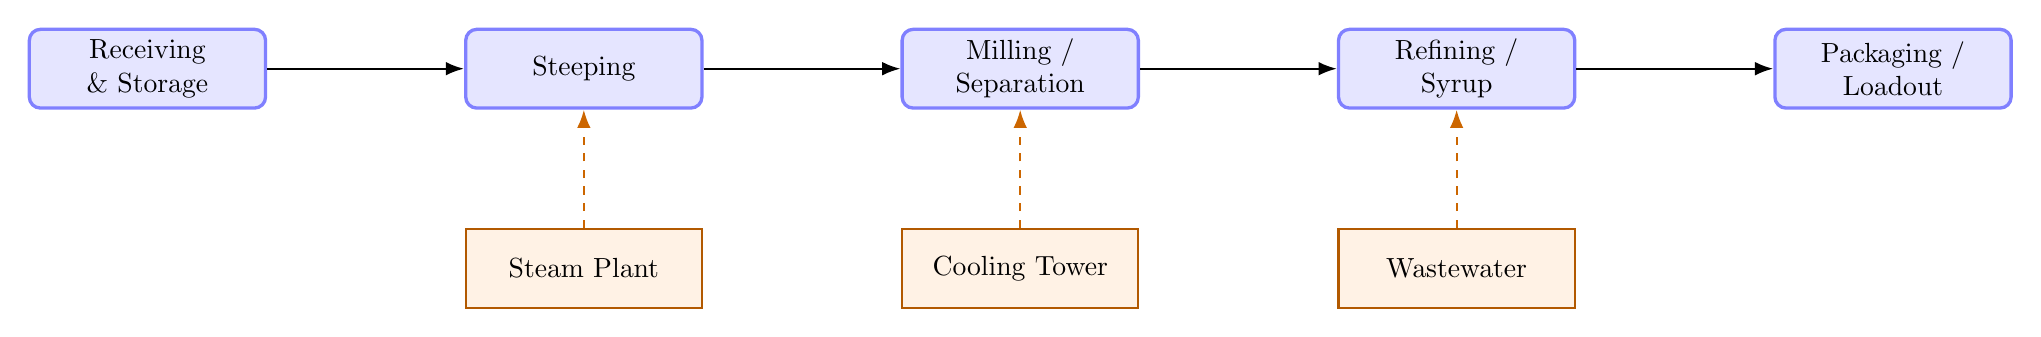
\begin{tikzpicture}[
  process/.style={rectangle, rounded corners, draw=blue!50, fill=blue!10, very thick, minimum width=3cm, minimum height=1cm, align=center},
  util/.style={rectangle, draw=orange!70!black, fill=orange!10, thick, minimum width=3cm, minimum height=1cm, align=center},
  arrow/.style={-Latex, thick}
]

\node[process] (recv) {Receiving \\ \& Storage};
\node[process, right=2.5cm of recv] (steep) {Steeping};
\node[process, right=2.5cm of steep] (mill) {Milling / \\ Separation};
\node[process, right=2.5cm of mill] (refine) {Refining / \\ Syrup};
\node[process, right=2.5cm of refine] (pack) {Packaging / \\ Loadout};

\node[util, below=1.5cm of steep] (steam) {Steam Plant};
\node[util, below=1.5cm of mill] (cool) {Cooling Tower};
\node[util, below=1.5cm of refine] (waste) {Wastewater};

\draw[arrow] (recv) -- (steep);
\draw[arrow] (steep) -- (mill);
\draw[arrow] (mill) -- (refine);
\draw[arrow] (refine) -- (pack);

\draw[arrow, dashed, orange!80!black] (steam) -- (steep);
\draw[arrow, dashed, orange!80!black] (cool) -- (mill);
\draw[arrow, dashed, orange!80!black] (waste) -- (refine);

\end{tikzpicture}
\end{document}
